\documentclass[10pt]{article}
\usepackage[a4paper,margin=2cm]{geometry}
\usepackage[T1]{fontenc}
\usepackage{lmodern,microtype,booktabs,tabularx,graphicx,amsmath,amssymb,xcolor,caption,subcaption}
\usepackage[hidelinks]{hyperref}
\usepackage{enumitem}
\setlist{nosep,leftmargin=*}
\captionsetup{font=small,labelfont=bf,skip=3pt}
\setlength{\parskip}{3pt}\setlength{\parindent}{0pt}
\setlength{\textfloatsep}{8pt plus 2pt minus 2pt}\setlength{\intextsep}{7pt plus 2pt minus 2pt}
\newcommand{\agOOV}{7.1\%}
\newcommand{\sstOOV}{7.0\%}
\newcommand{\gloveCov}{96.2\%}
\newcommand{\gloveTokCov}{95.9\%}
\newcommand{\gloveMissing}{1,098}
\newcommand{\wvTime}{82}
\newcommand{\rhoMean}{-0.7}
\newcommand{\rhoMeanP}{0.16}
\newcommand{\rhoLast}{-0.8}
\newcommand{\mcLstmRnnP}{0.44}
\newcommand{\mcTrEmbP}{0.44}
\newcommand{\bizSci}{515}
\newcommand{\allWrong}{532}
\newcommand{\gloveErrors}{1,170}
\newcommand{\pTrLstm}{0.004}
\newcommand{\meanrnn}{153.2}
\newcommand{\meanlstm}{135.0}
\newcommand{\meantransformer}{131.8}
\newcommand{\driftrnn}{0.98}
\newcommand{\drifttoprnn}{0.94}
\newcommand{\driftlstm}{0.98}
\newcommand{\drifttoplstm}{0.94}
\newcommand{\drifttransformer}{0.98}
\newcommand{\drifttoptransformer}{0.95}
\newcommand{\driftlstmsmall}{0.67}
\newcommand{\drifttoplstmsmall}{0.56}
\newcommand{\sdrnn}{0.2}
\newcommand{\sdlstm}{0.7}
\newcommand{\sdtransformer}{0.6}
\newcommand{\sdlstmwtwov}{1.9}
\newcommand{\sdlstmglove}{1.1}

\newcommand{\obs}{\textbf{Observation.}~}
\newcommand{\hyp}{\textbf{Possible explanation.}~}

\title{\vspace{-1.2cm}DSA4213 Assignment 1: Does Better Next-Token Prediction Give Better Representations?}
\author{Zhongze Zhao (A0357793J) \\ \small Code and \texttt{README.md}: \url{https://github.com/zzz84402816-lab/DSA4213-Assignment-1} (also submitted as a zip)}
\date{\vspace{-0.6cm}}

\begin{document}
\maketitle

\section{Question and setup}
\textbf{Comparison question.} I investigate whether stronger next-token prediction leads to more useful features
for topic classification. Part~I compares four language-model (LM) families using perplexity (PPL). Part~II keeps
the LSTM architecture fixed and varies its input embeddings. Part~III evaluates frozen representations on AG~News
and compares the downstream ranking with the language-model ranking.

\textbf{Corpus and preprocessing.} I use the official WikiText-2 v1 splits (\texttt{wikitext-2-v1}), containing
approximately 2.08M training, 216k validation and 244k test tokens. The release is already tokenised and replaces
rare words with \texttt{<unk>}. I lowercase the text for compatibility with uncased GloVe, remove empty lines and
add \texttt{<eos>} after each line. All models share a 28,913-entry vocabulary constructed only from training
tokens, including \texttt{<pad>}, \texttt{<unk>} and \texttt{<eos>}. Lowercasing introduces no additional
validation or test OOVs. The \texttt{<unk>} token accounts for 6.2\% of test tokens and is included in evaluation.

\textbf{Common evaluation.} All models follow the same evaluation protocol with non-overlapping 128-token windows
and state resets between windows. A prediction uses only the available preceding tokens within its window. There
are 244,101 test targets, with every test token after the first scored once. I right-pad the final window and
exclude padding targets from the loss. I report average cross-entropy (CE) in nats per non-padding token and
perplexity, calculated as $\mathrm{PPL}=\exp(\mathrm{CE})$. Checkpoints are selected using validation loss, and the
selected model is evaluated once on the test split.

\textbf{Models.} I compare four model families. The n-gram baseline is my interpolated Kneser--Ney implementation,
using an order-specific discount $D_k=n_1/(n_1+2n_2)$, lower-order continuation counts and a uniform base
distribution. Validation PPL was 274.8, 235.8 and 229.3 for orders 2, 3 and 4, so I selected the 4-gram. The RNN
and LSTM each use 300-dimensional embeddings, two 512-unit layers and a linear softmax output. The decoder-only
Transformer uses pre-layer normalisation, four layers, six heads, hidden size 300, FFN size 1200 and learned
positions. Its causal mask blocks future positions. A unit test for all three neural models verifies that changing
tokens at or after position $t$ does not affect earlier logits. The neural models share the same training settings:
trainable 300-dimensional embeddings initialised from $\mathcal N(0,1)$, dropout 0.3, context length 128 and batch
size 32. Each run lasts 20 epochs, approximately 10.1k steps or 41.5M target tokens. I use AdamW with learning rate
$10^{-3}$ and weight decay 0.01, followed by cosine decay after 300 warm-up steps, and clip gradients at 1.0. The
checkpoint with the lowest validation loss is retained. The primary runs use seed 42 and PyTorch 2.11 on a 12\,GB
RTX~5070~Ti Laptop GPU under WSL2.

\section{Part I: four language-model families}
\begin{table}[h]
\centering\small\setlength{\tabcolsep}{4pt}
\begin{tabular}{lrrrrrr}
\toprule
Model & Test CE & Test PPL & Test PPL & Train CE & Val CE & Gap \\
 & (nats) & seed 42 & 3 seeds & (eval mode) & & val$-$train \\
\midrule
KN 4-gram & 5.378 & 216.5 & (deterministic) & 2.10 & 5.44 & 3.33 \\
RNN & 5.033 & 153.4 & 153.2 $\pm$ 0.2 & 4.13 & 5.11 & 0.98 \\
LSTM & 4.905 & 135.0 & 135.0 $\pm$ 0.7 & 4.26 & 4.97 & 0.70 \\
Transformer & 4.876 & 131.0 & 131.8 $\pm$ 0.6 & 3.84 & 4.94 & 1.11 \\
\bottomrule
\end{tabular}
\\[3pt]
\begin{tabular}{lrrrrrrrrr}
\toprule
Model & Params & Non-emb & Train time & Train & Infer & \multicolumn{2}{c}{Gen ms/token} & Rep-3 & Dist-2 \\
 & (M) & (M) & s (s/epoch) & k tok/s & k tok/s & recomp. & increm. & greedy & top-$k$ \\
\midrule
KN 4-gram & 5.8$^\dagger$ & -- & 7 (CPU) & -- & 450 (CPU) & -- & 0.45 (CPU) & 0.55 & 0.93 \\
RNN & 24.4 & 0.94 & 433 (22/ep) & 105 & 274 & 2.82 & 0.43 & 0.34 & 0.92 \\
LSTM & 27.3 & 3.77 & 449 (22/ep) & 101 & 273 & 2.98 & 0.49 & 0.43 & 0.92 \\
Transformer & 21.8 & 4.37 & 384 (19/ep) & 126 & 484 & 1.36 & 1.51 & 0.41 & 0.90 \\
\bottomrule
\end{tabular}

\caption{Part I. Top: prediction quality and fit. \emph{3 seeds}: mean $\pm$ std of test PPL over seeds 42, 1, 2.
\emph{Train CE}: training split re-scored in eval mode (no dropout) with the selected weights, so that \emph{Gap}
= val CE $-$ train CE compares like with like. Bottom: cost and generation. \emph{Train time}: full 20-epoch budget, all three models re-trained in lockstep
(alternating order per epoch) so they share the same thermal conditions. \emph{Train/Infer k tok/s}:
round-robin benchmark (5 rounds, median; batch 32$\times$128). \emph{Gen}: model-only greedy decoding at batch 1,
120 new tokens, median of 5 round-robin rounds; \emph{recomp.} re-encodes the whole context each step,
\emph{increm.} carries the recurrent state or a key/value cache. \emph{Rep-3}: share of repeated trigrams in 40-token greedy
continuations; \emph{Dist-2}: distinct bigrams in top-$k$ samples (5 prompts $\times$10).
$^\dagger$stored $n$-gram count entries, not trainable parameters.}
\label{tab:p1}
\end{table}

\begin{figure}[h]
\centering
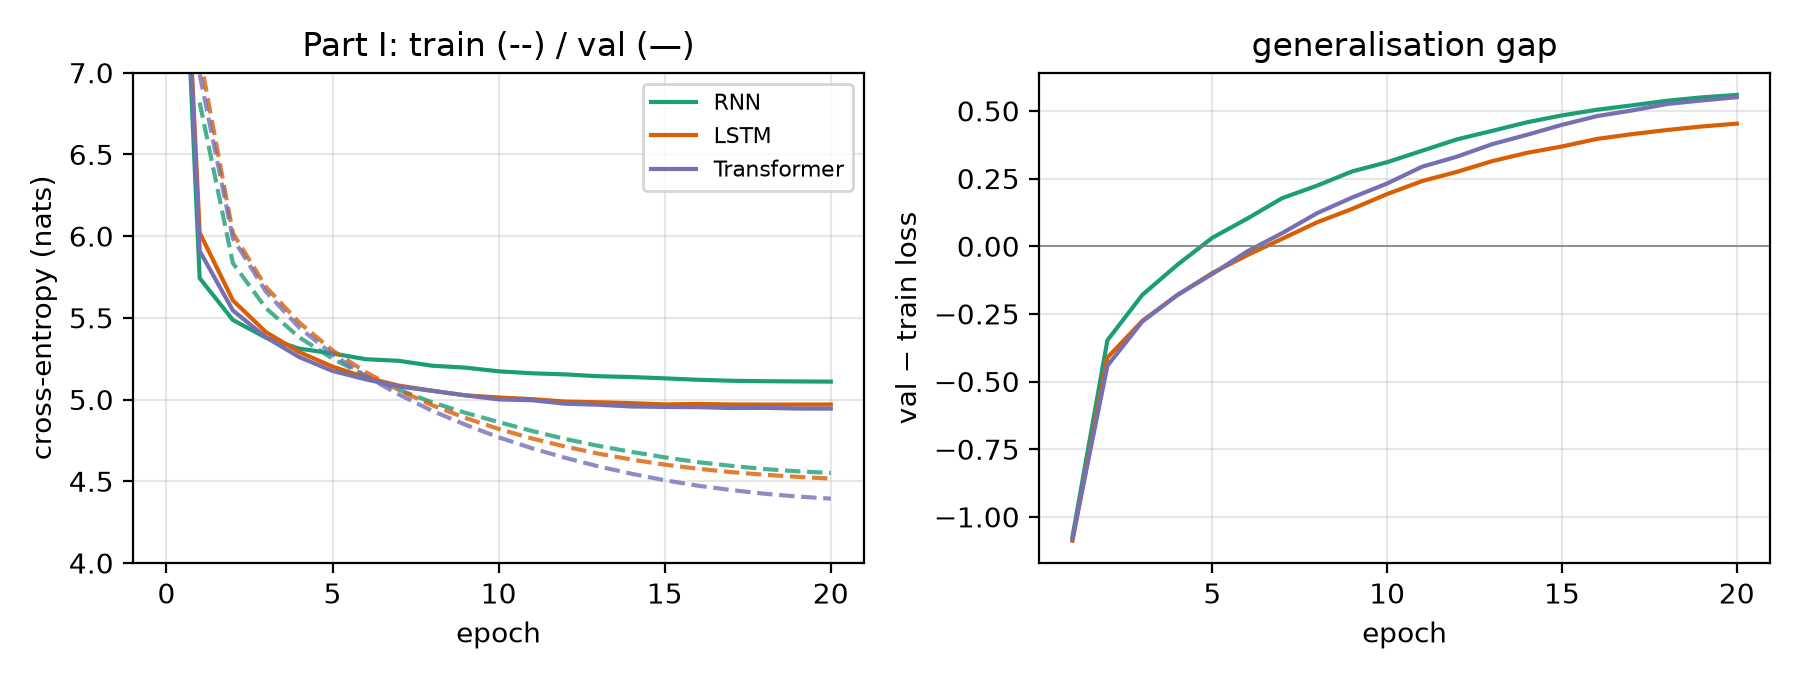
\includegraphics[width=0.76\linewidth]{../results/figures/part1_loss.png}
\caption{Part I training (dashed) and validation (solid) cross-entropy per epoch, and their difference. The logged
training loss is averaged over the epoch while the weights change and with dropout on, so it over-states the true
training loss: this is why the difference is \emph{negative} early on and why it under-states the final gap
(clean gaps at the selected checkpoint are in Table~\ref{tab:p1}).}
\label{fig:p1}
\end{figure}

\textbf{Prediction quality.} \obs The neural models all achieved substantially lower test PPL than the KN 4-gram.
Across three seeds, the order was Transformer (\meantransformer{} $\pm$ \sdtransformer), LSTM (\meanlstm{} $\pm$
\sdlstm), then RNN (\meanrnn{} $\pm$ \sdrnn), compared with 216.5 for the 4-gram. The Transformer had a small
advantage over the LSTM (Welch $t$-test $p$=\pTrLstm), while both were clearly ahead of the RNN. \hyp The 4-gram
relies on the previous three tokens and must back off when a context is unseen. Neural models can share information
through embeddings and access longer contexts. The RNN's lack of gates may make long-range information harder to
preserve. However, it also has fewer non-embedding parameters (0.94M versus about 3.8M and 4.4M), so this
comparison does not separate architecture from capacity.

\textbf{Learning behaviour.} \obs Figure~\ref{fig:p1} shows that the RNN improved quickly at first but reached a
plateau sooner than the other neural models. The LSTM's validation curve became nearly flat after about 12 epochs,
with its best checkpoint at epoch 19; the Transformer was still improving slightly at epoch 20. None showed an
upward validation trend. Nevertheless, evaluation-mode scoring revealed substantial val$-$train CE gaps
(Table~\ref{tab:p1}): \gaptr{} nats for the Transformer, \gaprnn{} for the RNN, \gaplstm{} for the LSTM and
\gapngram{} for the 4-gram. These gaps varied by at most 0.02 across seeds. \hyp The models fit training-specific
patterns that do not transfer fully to unseen text. Dropout and the learning-rate schedule may have helped, but
their effects were not tested separately. The Transformer combined the lowest validation loss with a larger gap
than the LSTM, showing that gap size alone does not determine test quality. Its unfinished learning curve suggests
that more training could help; the RNN's larger gap may reflect overfitting to local patterns in the training data
or hyperparameter settings that are less suitable for this architecture, although neither explanation has been
verified.

\textbf{Cost.} \obs Sequential training runs gave misleading wall-clock times on the laptop GPU (epoch times of the
\emph{same} model drifted from 21 to 33\,s as it heated up), so I measured cost under shared conditions. Re-training
the three models in lockstep for the full budget, the Transformer is the fastest to train (\lockTimeTr\,s vs.\
\lockTimeRnn\,s RNN and \lockTimeLstm\,s LSTM; it reaches the same validation loss as before), and the round-robin
benchmark agrees (training \bTrainTr k vs.\ \bTrainLstm--\bTrainRnn k tok/s; scoring \bInferTr k vs.\
\bInferLstm--\bInferRnn k tok/s). The KN model trains in \ngFitTime\,s on one CPU thread. \emph{Generation} reverses
the ranking. Re-encoding the context at every step, the RNN/LSTM cost grows with length (\genRnnRecShort{} $\to$
\genRnnRecLong{} ms/token for the RNN from 40 to 120 tokens) while the Transformer stays at \genTrRecShort--\genTrRecLong{}
ms. Carrying the recurrent state makes the RNN/LSTM constant at $\approx$\genRnnIncLong--\genLstmIncLong{} ms/token,
2.5--3$\times$ faster than the Transformer, whose key/value cache (\genTrIncLong{} ms) brings no gain at this
scale. \hyp Training and scoring see the whole window at once, which the Transformer parallelises across
positions while recurrent models must step through it; generation produces one token at a time, where an
$O(1)$ recurrent update is cheap. At batch 1 and $\le$128 tokens the GPU is mostly idle and latency is dominated by
per-operation launch overhead, so my unfused cache cannot beat PyTorch's fused full-context kernel; a fused cache
or longer contexts could change the Transformer's numbers, which I did not test.

\textbf{Generated text.} \obs With matched prompts and 40-token continuations (Table~\ref{tab:gen};
\texttt{<unk>} banned), greedy decoding caused repetition in every model. The repeated-trigram rate was highest for
KN (55\%) and lowest for the RNN (34\%). Top-$k$ sampling greatly reduced this behaviour. Some neural samples
contain recognisable clauses and military-related words, whereas the 4-gram often connects short, locally
plausible fragments. However, grammatical wording does not guarantee sensible content: \emph{``the royal fleet was
an apprentice officer''} is semantically inconsistent. Topic continuity is also unreliable beyond the opening
sentence. The neural models reproduce WikiText formatting, including headings and \texttt{<eos>}. Overall, these
samples suggest better local structure than sustained, meaningful discourse.
\emph{Blind rating.} I also scored \heItems{} randomly selected top-$k$ samples from each model after shuffling
them and hiding model identities (Table~\ref{tab:human}). Fluency and consistency used the 1--3 rubric in
\texttt{README.md}. No sample received the highest fluency score. Among Part~I models, the Transformer had the
highest mean consistency (1.70), while every 4-gram sample scored 1. Their difference was significant
(Mann--Whitney $p$=\heTrNgCon), but Transformer versus LSTM was not ($p$=\heTrLstmCon). Mean fluency scores of
1.2--1.6 did not establish a clear ordering. \hyp Better next-token prediction may improve short-range continuity
without ensuring discourse coherence. Limited data or capacity may contribute, but this experiment does not identify
the cause. The reduction in repetition under top-$k$ sampling indicates that decoding choice also matters. These
conclusions remain tentative because there was one rater and only \heItems{} samples per model.

\begin{table}[h]
\centering\footnotesize
\begin{tabularx}{\linewidth}{lX}
\toprule
\multicolumn{2}{l}{Prompt: \textit{during the second world war ,} \quad (top-$k$=40, $T$=0.8 unless noted; first sample, first 24 tokens)} \\
\midrule
KN 4-gram & and , unlike the most controversial of all the millennium stadium , but i just want to be with them , and the first \ldots \\
RNN & and did not have two different types of the solar family . \textlangle eos\textrangle in the late 20th century , many archaeologists were not only \ldots \\
LSTM & the royal fleet was an apprentice officer on the main naval brigade . he was appointed adjutant 's flagship by the british navy , \ldots \\
Transformer & the company took place off their first position in australia , where they suffered a new zealand brigade , they had been unable to \ldots \\
LSTM+GloVe & the largest had been estimated and was considered a high @-@ time @-@ known @-@ scale @-@ time @-@ long area . the first \ldots \\
KN 4-gram (greedy) & and the first to be released in the united states , and the first to be released in the united states , and the \ldots \\
Transformer (greedy) & the first world war ii was the first world war ii . the war was the first world war ii in the war , \ldots \\
\bottomrule
\end{tabularx}

\caption{Matched continuations (more in \texttt{results/generations.md}).}
\label{tab:gen}
\end{table}

\begin{table}[h]
\centering\footnotesize
\begin{tabular}{lrcc}
\toprule
Model & Test PPL & Fluency & Consistency \\
\midrule
KN 4-gram & 216.5 & 1.20 [1.0, 1.5] & 1.00 [1.0, 1.0] \\
RNN & 153.4 & 1.30 [1.0, 1.6] & 1.30 [1.1, 1.6] \\
LSTM & 135.0 & 1.30 [1.0, 1.6] & 1.20 [1.0, 1.5] \\
Transformer & 131.0 & 1.50 [1.2, 1.8] & 1.70 [1.3, 2.1] \\
LSTM + Skip-gram & 130.4 & 1.60 [1.3, 1.9] & 1.70 [1.3, 2.1] \\
LSTM + GloVe & 133.9 & 1.30 [1.0, 1.6] & 1.20 [1.0, 1.5] \\
\bottomrule
\end{tabular}

\caption{Blind human rating of top-$k$ samples (one rater, \heItems{} samples per model, 1--3 scale): mean and
bootstrap 95\% CI.}
\label{tab:human}
\end{table}

\section{Part II: input-embedding ablation (LSTM)}
\textbf{Design.} I vary the input embeddings of the LSTM, the stronger recurrent model in Part~I. Setting~1 reuses
the Part~I configuration with trainable random embeddings. Setting~2 uses frozen 300-dimensional Skip-gram vectors
trained only on WikiText-2's training split in gensim, with window size 5, five negative samples and 10 epochs.
They cover the full vocabulary and require \wvTime\,s on one CPU thread, excluded from LM training time. Setting~3
uses frozen GloVe 6B 300d vectors from Wikipedia 2014 and Gigaword~5. After the mappings
\texttt{@-@}$\to$\texttt{-}, \texttt{@,@}$\to$\texttt{,} and \texttt{'t}$\to$\texttt{n't}, coverage is
\gloveCov{} of vocabulary types and \gloveTokCov{} of training tokens. The \gloveMissing{} uncovered types receive
random $\mathcal N(0,\sigma^2)$ vectors, where $\sigma$ is GloVe's standard deviation; \texttt{<pad>} is zero. These
rows are frozen too. All remaining parameters are trained from scratch using the Part~I procedure. In addition to
seed 42, I repeat the runs with seeds 1 and 2.

\begin{table}[h]
\centering\small\setlength{\tabcolsep}{3.5pt}
\resizebox{\linewidth}{!}{\begin{tabular}{lrrrrrrrrr}
\toprule
Input embedding & Cover. & Train. & Test PPL & Test PPL & Val PPL & Val PPL & Ep. to & Gap & Step-loss \\
 & & (M) & seed 42 & 3 seeds & ep 1 & ep 3 & best+.05 & ep 20 & std \\
\midrule
Random $\mathcal{N}(0,1)$, trainable & -- & 27.3 & 135.0 & 135.0 $\pm$ 0.7 & 412 & 224 & 10 & 0.45 & 0.127 \\
Own Skip-gram, frozen & 100.0\% & 18.6 & 130.4 & 130.2 $\pm$ 1.9 & 559 & 239 & 11 & 0.40 & 0.123 \\
GloVe 6B, frozen & 96.2\% & 18.6 & 133.9 & 132.7 $\pm$ 1.1 & 564 & 237 & 11 & 0.33 & 0.122 \\
\textit{Suppl.:} random $\mathcal{N}(0,0.1^2)$, train. & -- & 27.3 & 140.3 & -- & 706 & 274 & 11 & 0.51 & 0.123 \\
\bottomrule
\end{tabular}
}
\caption{Part II. \emph{Cover.}: vocabulary types with a pretrained vector. \emph{3 seeds}: mean $\pm$ std over
seeds 42, 1, 2. \emph{Ep.\ to best+.05}: first epoch whose val loss is within 0.05 nats of the run's best.
\emph{Gap}: val $-$ train CE at the selected checkpoint, both scored in eval mode (as in Table~\ref{tab:p1}). \emph{Step-loss std}: mean within-epoch std of mini-batch loss.}
\label{tab:p2}
\end{table}

\begin{figure}[h]
\centering
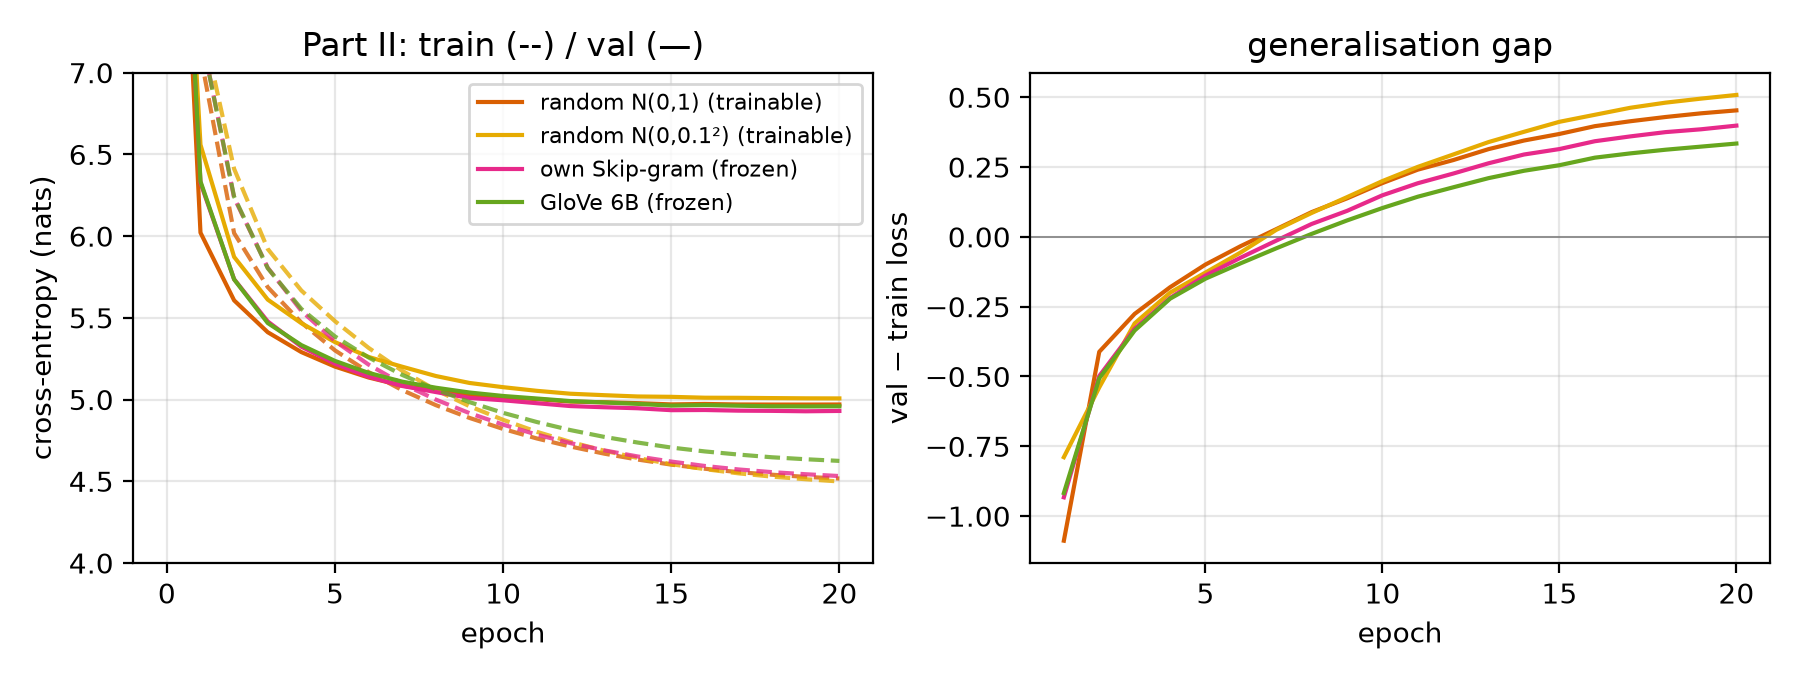
\includegraphics[width=0.76\linewidth]{../results/figures/part2_loss.png}
\caption{Part II learning curves (all LSTM, identical except the input-embedding table). As in Fig.~\ref{fig:p1},
the right panel uses the logged (dropout-on) training loss; clean gaps are in Table~\ref{tab:p2}.}
\label{fig:p2}
\end{figure}

\textbf{Results.} \obs (Table~\ref{tab:p2}, Fig.~\ref{fig:p2}) Across three seeds, frozen Skip-gram achieved the
best mean test PPL (130.2 $\pm$ \sdlstmwtwov), followed by frozen GloVe (132.7 $\pm$ \sdlstmglove) and trainable
random embeddings (135.0 $\pm$ \sdlstm). The mean improvements over the random baseline were 4.8 and 2.3 PPL,
respectively; the evidence is limited to three runs per setting. The random baseline improved faster initially
(epoch-1 validation PPL 412 versus about 560), but the frozen settings caught up around epoch 6. All reached within
0.05 nats of their best validation loss by epoch 10--11. Step-loss variability (0.122--0.127) and maximum gradient
norms (about 1.8) gave no clear stability advantage. GloVe had the smallest evaluation-mode val$-$train gap (0.57
versus 0.64 and 0.70 nats), together with the highest training loss. This is consistent with constrained fitting,
but a smaller gap alone does not imply better prediction: Skip-gram still had the lowest test PPL.
The generation metrics were similar across embedding settings: distinct-2 was 0.92, 0.91 and 0.90, and greedy
repeated-trigram rates were 0.43, 0.49 and 0.47 for random, Skip-gram and GloVe. None reliably maintained coherent
content. The \texttt{@-@} chain in the displayed GloVe sample (Table~\ref{tab:gen}) was not unique to GloVe: among
the 50 samples per model, such chains occurred 4 times for GloVe, 4 for Skip-gram, 0 for the random-embedding LSTM
and 3 for the RNN. These counts do not establish whether embedding choice affects the behaviour. In the blind
ratings (Table~\ref{tab:human}), Skip-gram had higher mean consistency (1.70) than GloVe or the random baseline
(both 1.20), but the Skip-gram--GloVe comparison was not significant ($p$=\heSgGloveCon). With \heItems{} rated
samples per model, I treat this as a tentative pattern rather than a reliable ranking.

\textbf{Why does ``trainable'' not win?} \obs The default trainable embeddings changed little in direction: the mean
initial-to-final cosine was \driftlstm{} for all three neural models, and \drifttoplstm{} for the LSTM's 1,000 most
frequent words. Their nearest neighbours remained largely unrelated in meaning, unlike those from Skip-gram or GloVe
(Appendix Table~\ref{tab:nn}). \hyp The initial vectors had large norms, about 17, which may have made the learned
changes small relative to the starting vectors. However, the learning rate alone does not determine the accumulated
AdamW update, and cosine similarity measures direction rather than total change. The evidence therefore supports
limited semantic reorganisation, not the claim that the embeddings were effectively unchanged. Adaptation may also
occur in later layers. Part~III further shows that even these small directional changes can improve topic features.
\emph{Supplementary test:} with a smaller initialisation, $\mathcal N(0,0.1^2)$, the embeddings changed more in
direction (mean cosine \driftlstmsmall; \drifttoplstmsmall{} for frequent words) and developed some meaningful
neighbours, such as \emph{king}--\emph{queen} and \emph{football}--\emph{rugby}. This did not improve language
modelling within 20 epochs: test PPL increased to 140.3. Training CE was also higher (4.30 versus 4.26), while the
val$-$train gap was almost unchanged (0.71 versus 0.70). Together with slower early learning (epoch-1 validation PPL
706 versus 412) and continued improvement at epoch 20, this pattern is more consistent with slower optimisation than
increased overfitting. Smaller inputs may contribute, but that mechanism was not directly tested. A longer run might
help, although this remains unverified. Despite its worse PPL, this model produced better downstream features in
Part~III.

\textbf{Interpretation.} The random and pretrained settings differ in both embedding training history and whether
the table is updated during LM training. Comparing frozen Skip-gram with frozen GloVe holds trainability fixed, but
it does not isolate a single cause: the tables also differ in learning method, corpus size, domain and coverage. In
these runs, in-domain Skip-gram gave lower WikiText-2 PPL than GloVe despite using far less text. Thus, more
pretraining data did not guarantee better performance on this LM objective. GloVe performed better on AG News in
Part~III, but that result cannot be attributed to data quantity alone.
\emph{Leakage check:} because WikiText-2 and part of GloVe's pretraining corpus both come from Wikipedia, overlap
with the WikiText-2 test articles is possible. The experiment does not verify the exact overlap. Frozen word vectors
encode corpus statistics rather than explicit test sequences, but this does not rule out information from
overlapping data. GloVe's failure to outperform train-only Skip-gram also does not prove that overlap had no effect.
I therefore treat the GloVe setting as potentially affected by pretraining overlap. The Skip-gram setting provides
the cleaner comparison because its vectors were trained only on the designated WikiText-2 training split.

\section{Part III: frozen LM representations for AG News}
\textbf{Task and data.} The downstream task is four-class AG News topic classification: World, Sports, Business and
Sci-Tech. I sample 20,000 training articles with equal class counts and evaluate on all 7,600 official test
articles. A rule-based tokenizer follows WikiText conventions, including forms such as \texttt{didn 't} and
\texttt{3 @.@ 5}. Using the WikiText-2 vocabulary, the AG News test-token OOV rate is \agOOV, close to SST-2's
\sstOOV, so this coverage measure did not determine the choice. I chose AG News because its register is reasonably
close to Wikipedia and it provides a large labelled test set; SST-2's test labels are not public.

\textbf{Representations.} For each frozen LM, I truncate articles to 128 tokens and right-pad shorter inputs. I
extract three representations: \emph{Last} uses the top-layer state at the final non-padding token; \emph{Mean}
averages top-layer states over non-padding positions; \emph{Emb} averages the input embeddings without contextual
processing. Emb serves as a reference for assessing what the contextual layers contribute. Each representation uses
the same standardisation and multinomial logistic-regression pipeline. I select $C$ from $\{10^{-3},\dots,1\}$ using
macro-F1 on a 10\% validation portion of the training subset, then refit on all 20,000 training examples. The
language models remain frozen throughout.

\begin{table}[h]
\centering\small\setlength{\tabcolsep}{4pt}
\begin{tabular}{lcrccc}
\toprule
Frozen LM & Seeds & LM test & Last state & Mean of states & Mean of input emb. \\
 & & PPL & \multicolumn{3}{c}{test accuracy (mean $\pm$ std over LM seeds)} \\
\midrule
RNN & 3 & 153.2 & 0.616\,{\scriptsize$\pm$0.001} & 0.713\,{\scriptsize$\pm$0.006} & 0.759\,{\scriptsize$\pm$0.004} \\
LSTM & 3 & 135.0 & 0.650\,{\scriptsize$\pm$0.010} & 0.710\,{\scriptsize$\pm$0.008} & 0.740\,{\scriptsize$\pm$0.006} \\
Transformer & 3 & 131.8 & 0.730\,{\scriptsize$\pm$0.010} & 0.772\,{\scriptsize$\pm$0.007} & 0.772\,{\scriptsize$\pm$0.004} \\
LSTM + Skip-gram (frozen) & 3 & 130.2 & 0.767\,{\scriptsize$\pm$0.009} & 0.802\,{\scriptsize$\pm$0.003} & 0.824$^\ddagger$ \\
LSTM + GloVe (frozen) & 3 & 132.7 & 0.794\,{\scriptsize$\pm$0.004} & 0.844\,{\scriptsize$\pm$0.002} & 0.878$^\ddagger$ \\
\midrule
\textit{Suppl.:} LSTM, $\mathcal{N}(0,0.1^2)$ init & 1 & 140.3 & 0.644 & 0.731 & 0.765 \\
\textit{Control:} untrained LSTM & -- & 28,975 & 0.475 & 0.718 & 0.683 \\
\textit{Control:} untrained Transformer & -- & 32,833 & 0.496 & 0.650 & 0.683 \\
\midrule
\textit{Reference:} TF-IDF bag of words, no LM & -- & -- & \multicolumn{3}{c}{0.885} \\
\bottomrule
\end{tabular}

\caption{Part III test accuracy on 7,600 AG News test articles (macro-F1 is within \maxFdiff{} of accuracy in every
cell). Trained LMs: mean $\pm$ std over the three LM seeds used in Parts I--II. $^\ddagger$frozen pretrained table, hence
identical for all seeds. \emph{Controls}: the seed-42 \emph{initial} weights of the LSTM/Transformer, never trained
(both share the same initial embedding table). With $n$=7,600 the standard error of an accuracy near 0.8 is
$\approx$0.005; exact McNemar tests (seed-42 models) are in \texttt{results/downstream/error\_stats.json}.}
\label{tab:p3}
\end{table}

\begin{figure}[h]
\centering
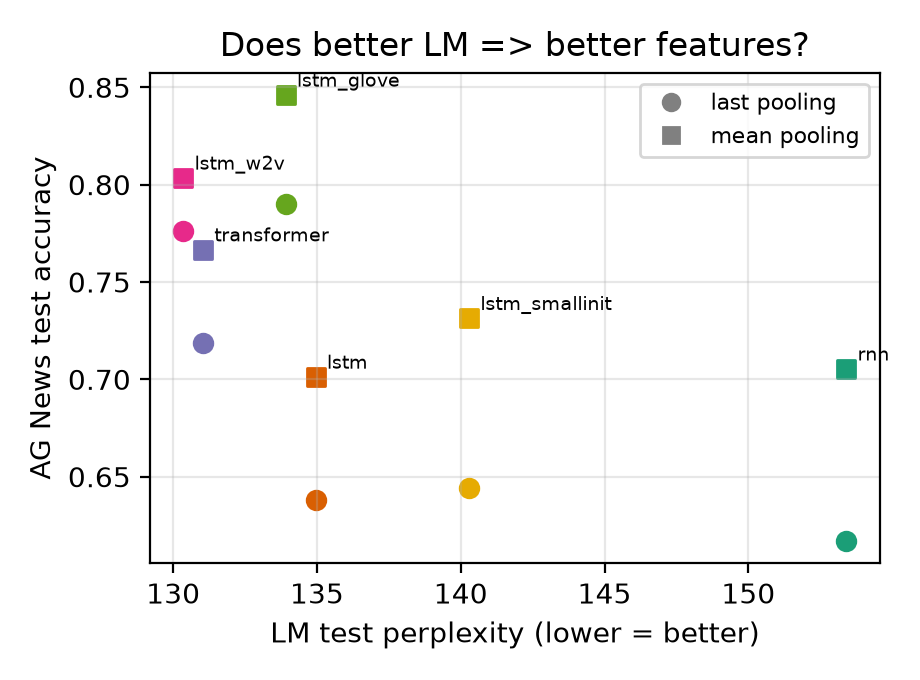
\includegraphics[width=0.82\linewidth]{../results/figures/part3_ppl_vs_acc.png}
\caption{LM test perplexity vs.\ downstream accuracy, one point per trained checkpoint (3 seeds per family).}
\label{fig:p3}
\end{figure}

\textbf{Which representation works better?} \obs (Table~\ref{tab:p3}, Fig.~\ref{fig:p3}) Mean pooling outperformed
the last state for every trained LM; for the LSTM, accuracy was \accLstmMean{} versus \accLstmLast{} (seed-42
McNemar $p<10^{-28}$). Among the Part~I models, the Transformer had the strongest mean-pooled features
(\accTrMean{} versus \accLstmMean{} for the LSTM; seed-42 $p<10^{-37}$). The RNN and LSTM had similar accuracy
despite an 18-point PPL difference. Frozen pretrained embeddings improved the LSTM results to \accSgMean{} with
Skip-gram and \accGloveMean{} with GloVe. The single small-init run also improved on the default LSTM
(\accSmallMean{} versus \accLstmMean{} $\pm$ \sdLstmMean), despite worse PPL. However, averaging input embeddings
matched or exceeded averaging contextual states in every trained model; GloVe reached \accGloveEmb{} versus
\accGloveMean. TF-IDF was numerically highest at \bowAcc. For this topic task, these results suggest that lexical
information is particularly useful and that contextual processing does not automatically improve a pooled
representation.

\textbf{Does LM training help the features at all?} \obs Compared with the untrained controls (test PPL
\pplUnLstm{} / \pplUnTr), training improved the last-state features substantially: accuracy rose from
\accUnLstmLast{} to \accLstmLast{} for the LSTM and from \accUnTrLast{} to \accTrLast{} for the Transformer. The
Transformer's mean-pooled accuracy rose from \accUnTrMean{} to \accTrMean. Input-embedding averages also improved,
from \accUnLstmEmb{} to \accLstmEmb--\accTrEmb, so the small directional drift in Part~II was still useful for topic
classification. In contrast, the untrained LSTM's mean pooling reached \accUnLstmMean, close to the trained result
of \accLstmMean{} $\pm$ \sdLstmMean. \hyp Averaging random LSTM states may preserve enough lexical information for a
linear classifier to recognise topics. Next-token training need not improve that particular summary. This is a
possible mechanism, not evidence that random LSTM states are literally a linear projection of word counts. The
untrained Transformer mean was weaker than its embedding average (\accUnTrMean{} versus \accUnTrEmb), suggesting
less accessible lexical information after random contextual processing. Pretrained vectors and GloVe's news-domain
exposure offer another possible source of useful topic information.

\textbf{Does PPL rank agree with downstream rank?} \obs Across \nAll{} trained checkpoints, lower PPL was associated
with higher accuracy: Spearman $\rho=\rhoAllMean$ for mean pooling ($p$=$\rhoAllMeanP$) and $\rho=\rhoAllLast$ for
the last state ($p$=$\rhoAllLastP$). The six seed-42 models alone gave weaker statistical evidence
($\rho=\rhoMean$, $p$=\rhoMeanP). Within Part~I, the association was clearer for the last state ($\rho=\rhoPILast$,
$p$=$\rhoPILastP$) than for mean pooling ($\rho=\rhoPIMean$, $p$=\rhoPIMeanP). Nevertheless, PPL did not
consistently rank individual settings. RNN and LSTM had similar mean-pooled accuracy despite an 18-point PPL gap;
small initialisation improved accuracy while worsening PPL; and GloVe improved accuracy by about four percentage
points over Skip-gram despite PPL being 2.5 higher. These counterexamples show that PPL is not a sufficient
selection criterion for this downstream task. Because the checkpoints include repeated seeds within a few model
settings, the correlation should be read as a pattern in this experiment, not a universal relationship.

\textbf{Error analysis.} \obs In the seed-42 results, Business and Sci/Tech were the main source of confusion. They
accounted for \bizSci{} of the GloVe-LSTM's \gloveErrors{} errors. Headlines about technology companies' finances,
such as Dell leaving a PC market or IBM reporting revenue growth, plausibly fit both topics. All five main LM systems
misclassified the same \allWrong{} articles, including some with debatable labels. Cases corrected by GloVe often
contained news-related proper nouns such as \emph{Isinbayeva}, \emph{DaimlerChrysler}, \emph{Linux} and
\emph{Dalai Lama}. These examples suggest a possible vocabulary advantage, but do not establish which words caused
the prediction. GloVe-LSTM accuracy was 0.82 in the shortest-length quartile and 0.85--0.86 in the others. Accuracy
did not decrease with a higher \texttt{<unk>} share (Appendix Table~\ref{tab:oov}). Remaining words may provide
enough topic information, although differences between the article groups could also explain this pattern.
Business had the lowest recall for every model.

\section{Connecting the parts, limitations, and lessons}
\textbf{Answer to the question.} Better next-token prediction was associated with better representations overall,
but it was not a reliable rule for choosing features. Across \nAll{} trained checkpoints, mean-pooled accuracy
correlated negatively with PPL ($\rho=\rhoAllMean$), and the Transformer led the random-embedding models on both
measures. However, RNN versus LSTM, small versus default initialisation, and GloVe versus Skip-gram all showed that
a PPL improvement need not translate into an accuracy improvement. The strong embedding-average and TF-IDF results
suggest that lexical information is especially useful for AG News. LM training improved several representations,
but added little to the LSTM's mean-pooled accuracy in the tested setup. GloVe's downstream advantage may reflect
pretraining data and domain match, which this experiment cannot separate. The practical conclusion is to evaluate
features on the downstream task directly. In the controlled neural-model benchmark, the Transformer also had the
highest training and scoring throughput, although the recurrent models generated faster one token at a time.

\textbf{Limitations.} The findings are limited to one roughly 2M-token LM corpus and a 20-epoch budget. The
Transformer's continuing improvement suggests that more training could change the results, but does not establish
how the ranking would change. All Part~I neural models used $\mathcal N(0,1)$ embeddings and showed little
directional drift; using the same initialisation does not guarantee an equal effect on different architectures. The
main neural settings used three seeds, while the small-init experiment and untrained controls used one. Laptop
thermal conditions also limit timing precision, despite the lockstep and round-robin protocols. Downstream
evaluation used frozen features and a linear classifier on AG News, so other tasks or fine-tuning may give different
rankings. Human evaluation involved one rater and \heItems{} samples per model, limiting the strength of small
differences. Finally, GloVe differs in data quantity, domain and training method. Its news corpus overlaps AG News's
period and domain, and its Wikipedia corpus may overlap WikiText-2; exact article overlap was not checked.

\textbf{Lessons.} This experiment taught me to compare computational cost under matched measurement conditions and
to calculate the generalisation gap using training and validation losses scored in the same mode. Re-scoring the
training set changed the interpretation of the small-init run. I also learned to inspect how trainable embeddings
change, rather than treating the trainable label as evidence of useful learning. Most importantly, representation
quality needs its own downstream evaluation: a lower language-model PPL is informative, but is not enough to select
the best features.

\clearpage
\appendix
\section*{Appendix}
\begin{table}[h]
\centering\footnotesize
\begin{tabularx}{\linewidth}{lXXX}
\toprule
Word & LSTM (random, learned) & Skip-gram (own) & GloVe 6B \\
\midrule
\textit{king} & posse, designer, bishop, schoolmaster & veera, æthelred, leinster, ballala & queen, prince, monarch, kingdom \\
\textit{war} & mart, [non-Latin] kalachuris, 1850 & outbreak, civil, liberties, airbase & wars, conflict, battle, civil \\
\textit{football} & ace, universal, joker, jallon & athletic, f.c., premier, varsity & soccer, basketball, league, baseball \\
\textit{france} & outreach, blazers, chivo, cups & italy, germany, sweden, russia & french, paris, belgium, spain \\
\textit{album} & crush, roxas, predict, carey & slayer, albums, yankovic, furtado & albums, song, ep, band \\
\textit{good} & eaten, 1972, radial, outstandingly & sublime, shocking, exciting, naive & better, really, always, you \\
\bottomrule
\end{tabularx}

\caption{Cosine nearest neighbours in four 300-d input-embedding tables (LSTM columns: tables after LM training
with default and small initialisation).}
\label{tab:nn}
\end{table}

\begin{table}[h]
\centering\footnotesize
\begin{tabular}{lrrrr}
\toprule
\texttt{<unk>} share & 0 & (0,5\%] & (5,10\%] & >10\% \\
Articles & 838 & 2122 & 2686 & 1954 \\ \midrule
LSTM (mean) & 0.660 & 0.713 & 0.696 & 0.714 \\
Transformer (mean) & 0.741 & 0.774 & 0.759 & 0.779 \\
LSTM + GloVe (frozen) (mean) & 0.828 & 0.850 & 0.846 & 0.850 \\
\bottomrule
\end{tabular}

\caption{AG News test accuracy by the share of \texttt{<unk>} tokens in an article (mean pooling).}
\label{tab:oov}
\end{table}

\textbf{Reproduction.} \texttt{scripts/run\_all.sh} regenerates every number, table and figure; all tables in this
report are produced by \texttt{src/latex\_tables.py} from \texttt{results/}.

\section*{References, sources and tool use}
\textbf{Tools and sources.} WikiText-2 (Merity et al., 2017), GloVe (Pennington et al., 2014), AG News (Zhang et
al., 2015), SST-2 (Socher et al., 2013) via HuggingFace \texttt{datasets} / \texttt{gensim}; PyTorch, gensim,
scikit-learn. Kneser--Ney follows Chen \& Goodman (1999). Code structure adapted from the DSA4213 course
notebooks. \textbf{AI assistance:} I used Claude Code (Anthropic) as a coding assistant for code
scaffolding, debugging, running experiments and drafting parts of this report, and ChatGPT (OpenAI, astra6) to help
rewrite and edit the analysis text in my own words; the free-text note column of the rating sheet was filled by an
AI tool from my scores and is not used in the analysis (all ratings are my own). All numbers are produced
by the submitted code; I checked them against the result files and the interpretation reflects my own understanding.

\textbf{References.}
Chen \& Goodman (1999), An empirical study of smoothing techniques for language modeling, \emph{CSL}.
Merity et al.\ (2017), Pointer sentinel mixture models, \emph{ICLR}.
Pennington et al.\ (2014), GloVe, \emph{EMNLP}.
Socher et al.\ (2013), Recursive deep models for semantic compositionality, \emph{EMNLP}.
Zhang et al.\ (2015), Character-level convolutional networks for text classification, \emph{NeurIPS}.
\end{document}
